% !TEX encoding = UTF-8
% !TEX TS-program = pdflatex
% !TEX root = ../tesi.tex

%**************************************************************
\chapter{Processi e metodologie}
\label{cap:processi-metodologie}
%**************************************************************

\intro{Brevissima introduzione al capitolo}\\

%**************************************************************
\section{Processo sviluppo prodotto}
Durante ogni attività è stata seguita una metodologia di sviluppo \gls{agileg}. L'azienda iVoxIT S.r.l. per la precisione attua in ogni suo progetto il metodo \gls{scrumg}. Le attività sono state descritte in task secondo la modalità \gls{scrumg}; ogni task veniva esposto e discusso in riunioni giornaliere con il tutor aziendale Dott. Sara Meneghetti. Inoltre erano previste riunioni settimanali con il responsabile del progetto Ing. Roberto Griggio.

\subsection{Metodologie di sviluppo Agile}
Le metodologie di sviluppo agile si basano su quattro principi cardine:
\begin{itemize}
    \item il software funzionante prima dei documenti;
    \item il rapporto con il cliente;
    \item i rapporti interno al team;
    \item rispondere al cambiamento;
\end{itemize}

Dal momento che i processi di pianificazione necessari ad uno sviluppo a cascata sono molto costosi e, che se questi non vengono rispettati, tutta la pianificazione deve essere completamente rivista, queste metodologie si basano su modelli incrementali. Gli approcci agile tendono a progettare il minimo indispensabile in modo tale da essere sempre più reattivi e proattivi possibili agli inevitabili. Inoltre scrivere del software incrementale permette una progettazione iniziale molto snella, la quale con l’accrescere della conoscenza sul dominio può diventare sempre affinata. Tutto ciò rende meno costoso il refactoring del codice e anche l’inserimento di nuove funzionalità. 
Questi metodi sono adatti per piccoli team, molto coesi e uniti, e non dislocati in regioni diverse, questo perchè la comunicazione di persona è fondamentale. A tal proposito il team in cui ero inserito si componeva di tre membri.
Un altro punto critico è che essendo l’approccio alla comprensione dei requisiti e alla progettazione poco concentrato all’inizio e molto diluito in tutto il progetto questo rende necessario un costante interesse da parte degli \gls{stakeholderg}, cosa che in un nuovo progetto è ipotizzabile, mentre in un progetto in fase manutentiva no.
\subsection{Scrum}
Scrum è un metodo iterattivo che divide il progetto in blocchi rapidi di lavoro chiamati
Sprint, della durata massima di quattro settimane. Alla fine di ogni Sprint si ottiene
un incremento del prodotto e durante ogni fase dello stage si è seguito questo modello. 
Scrum prevede una prima fase di analisi e progettazione di massima e una successiva suddivisione del lavoro in unità’ creabili e implementabili in un unico sprint che poi vengono messi in un backlog. Prima di ogni sprint si sceglie una selezione di lavori in base alle priorità e si inseriscono nel backlog dello sprint. Gli sprint durano da 1 a 4 settimane e se il lavoro non viene portato a termine non viene prolungato lo sprint, ma rimesso nel backlog principale. Da ciò emerge come sia importante dare il giusto quantitativo di lavoro. È compito dello
Scrum Master assicurarsi del rispetto dei tempi, infatti quest' ultimo effettua quotidianamente una breve
riunione, della durata di circa quindici minuti, per valutare i progressi fatti (Daily
Scrum). I rapporti tra i membri del progetto sono stati importanti e per questo Scrum prevede riunioni giornaliere per rimanere aggiornati sullo stato dei lavori di ogni componente.
In Figura ~\ref{fig:scrum} è mostrato un tipico ciclo Scrum.
\begin{figure}[!h]   
    \centering
    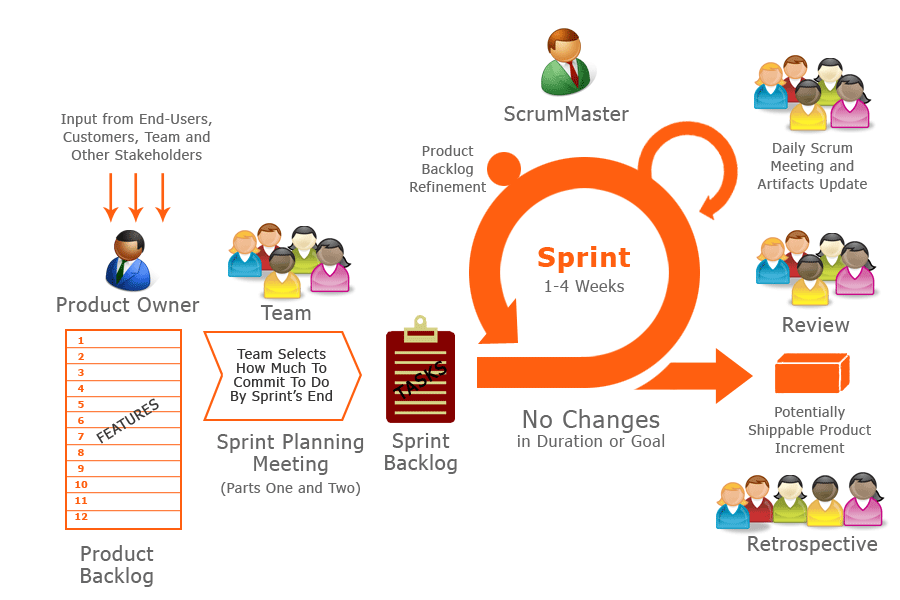
\includegraphics[width=0.9\columnwidth]{dig-scrum.png} 
    \caption{Diagramma flusso Scrum}
    \label{fig:scrum} 
\end{figure}